% Final report template; verified result macros are generated only after the final run completes.
\documentclass[10pt,a4paper]{article}
\usepackage[margin=.56in,top=.46in,bottom=.48in]{geometry}
\usepackage[T1]{fontenc}
\usepackage{mathptmx,amsmath,amssymb,booktabs,graphicx,microtype,xcolor,hyperref}
\definecolor{ink}{HTML}{234C72}
\hypersetup{colorlinks=true,urlcolor=ink,citecolor=ink,linkcolor=ink}
\setlength{\parindent}{0pt}\setlength{\parskip}{2.5pt}\setlength{\emergencystretch}{1.5em}
\newcommand{\sect}[1]{\par\vspace{4pt}{\color{ink}\fontsize{11}{12}\selectfont\bfseries #1}\par\vspace{1pt}}
\newcommand{\captext}[1]{{\footnotesize #1}\par}
\newcommand{\ind}{\mathbf1}
% Generated from completed final evidence by assets/bind_results.py.
\newcommand{\AbstractResult}{On 10,000 paired test scenarios, 54 of 55 Bonferroni-adjusted return contrasts favor the ensemble; the tuned diagnostic rule remains an unresolved rival with a better point estimate.}
\newcommand{\TrainingCompute}{Logged training totals 63.4 worker-minutes on CPU (five parallel workers, one Torch thread each).}
\newcommand{\InferenceMethod}{The 55 primary contrasts cover 22 comparator methods plus 33 fixed baseline checkpoints. A 50,000-resample bootstrap shares scenario draws while independently resampling actual comparator seed axes; the ensemble has one fixed-policy row. Bonferroni intervals use $\alpha=.05/55$. Secondary intervals use 2,000 resamples and are exploratory.}
\newcommand{\PrimaryResults}{The deployment obtains mean return $-1.637$ (nominal 95\% CI $[-1.725,-1.552]$). The strongest learned comparator, the final-checkpoint graph ensemble ($-2.174$), has paired deficit $0.537$ (simultaneous CI $[0.429,0.646]$). The matched temporal graph ensemble gives $-2.213$; the paired gain is $0.576$ ($[0.459,0.695]$). Fifty-four contrasts have positive adjusted lower bounds. 

The exception is the tuned diagnostic rule ($-1.557$): ensemble minus rule is $-0.081$ (adjusted CI $[-0.223,0.063]$). This comparison is inconclusive; universal superiority and equivalence are not established. The five individual final models average $-2.112$ with seed SD $0.213$; they are separate from the deployed ensemble.}
\newcommand{\SecondaryResults}{Uncontained hosts average $0.0252$ per episode. Explicit-confirmation coverage is only $8.62\%$ (nominal CI $[8.10,9.18]\%$), versus $88.53\%$ for the alert rule. Censored confirmation delay is $43.90$ versus $5.57$ steps. Low successful confirmation is a substantive weakness despite the return gains. The tuned rule has fewer uncontained hosts ($0.0097$) but more clean-host isolations ($0.2633$ versus $0.1656$); these are exploratory mean comparisons.}
\newcommand{\MetricTable}{Temporal DDQN & $-1.637$ & $0.0633$ & $0.1656$ & $8.62$ \\
Tuned diagnostic & $-1.557$ & $0.0729$ & $0.2633$ & $8.80$ \\
Graph final ens. & $-2.174$ & $0.0610$ & $0.2110$ & $9.84$ \\
Original threshold & $-2.750$ & $0.1085$ & $0.0418$ & $30.98$ \\
Original transfer & $-4.960$ & $0.2696$ & $0.0190$ & $92.65$ \\
Alert rule & $-11.527$ & $0.6043$ & $0.0000$ & $88.53$ \\}

\begin{document}
\begin{center}
{\Large\bfseries SentinelRL: Budgeted Network Defence with Deep RL}\par\vspace{4pt}
{\small\textbf{Rohit Mourya (B23ES1029)}\quad\textbf{Jyotiraditya Singh Rathore (B23ES1017)}}\par
{\small\href{https://github.com/rohitkumarmourya-maker/SentinelRL}{\texttt{github.com/rohitkumarmourya-maker/SentinelRL}}}\par
\end{center}
\small\textbf{Abstract.} SentinelRL allocates scarce defensive interventions in a synthetic network with stochastic attack propagation and noisy alerts. An exact public-history belief filter feeds a learned dueling Double DQN; a fixed temporal ensemble averages ten checkpoints from five training runs. The environment rewards critical-asset protection while penalizing damage, delayed confirmation and unnecessary isolation. \AbstractResult\ The claims concern this fixed deployment and prespecified test, with diagnosis and service trade-offs assessed separately.
\vspace{4pt}\hrule\vspace{3pt}
\begin{minipage}[t]{.482\textwidth}\vspace{0pt}\small
\sect{1. Task and stochastic environment}
A defender has $ B_0=6 $ response tokens over $ T=48 $ steps. An intervention changes future exposure, observations and remaining resources, making the task sequential rather than a static alert-classification problem. Six hosts have fixed attributes
\[
\begin{aligned}
v&=(.40,.68,.58,.82,.76,.48),\\
c&=(.45,.62,.80,1,.52,.96),
\end{aligned}
\]
with $c_i\geq.80$ defining critical assets. Undirected edges are $(0,1)$, $(1,2)$, $(2,3)$, $(1,4)$, $(4,2)$, $(3,5)$ and $(2,5)$.

Initially one hidden foothold is at host 0 with probability $.62 $, otherwise host 4. A compromised, unisolated source attempts to infect each susceptible, unisolated neighbour $ j $ with probability
\[
q_j=.23v_j(.20)^{p_j}(.25)^{d_j},
\]
where $ p_j,d_j $ mark patch/decoy deployment. Sources are snapshotted: new infections spread on the next step. Isolation blocks incoming/outgoing movement; patch and decoy reduce risk without curing infection. Nonisolated hosts emit binary alerts with sensitivity $.55 $ and false-positive rate $.08 $. Independent pre-sampled noise supports paired comparisons. No real network traffic or adaptive attacker is modeled.
\sect{2. State, observation and causal belief}
The augmented reward-relevant state has 56 dynamic entries: per host, compromise, patch, isolation, decoy, alert, alert EWMA, last inspection result/time and ever-confirmed flag, plus budget/time. The hidden compromise pattern $ z\in\{0,1\}^6 $ has 64 possibilities. Graph, $ v,c $ are constants.

Public observation $ o_t\in[0,1]^{56}$ has nine entries per host (alert, EWMA, last inspection result, normalized inspection age, $ v,c $, patch, isolation, decoy), plus $ B_t/6,t/48 $. Results encode unknown/clean/compromised as $ 0/.5/1 $ and remain stale after hidden infection; EWMA weight is $.35 $. No true infection count or actual entry identity is exposed.

Using only public action/alert/inspection history $ h_t $, maintain $ b_t(x)=P(z_t=x\mid h_t)$ over 64 patterns~\cite{pomdp}. For an explicit inspection of $ i $ returning $ e $, let $ g_t(x)=\ind[x_i=e]$; otherwise $ g_t=1 $. Then
\[
b_{t+1}(x')\propto\Omega(y_{t+1}\mid x')\sum_xP_{a_t}(x'\mid x)b_t(x)g_t(x).
\]
Inspection conditions the pre-spread state; action-updated public defenses determine the transition, followed by the new alarm likelihood. Isolated sensors are ignored. Reset conditions the $.62/.38 $ prior on initial alerts. Exactness assumes the known synthetic law. The Q input $\xi_t\in[0,1]^{126}$ contains public/history features 56, joint posterior 64 and marginals 6. Raw alert/EWMA/age slots are zeroed; the inspection-result slot becomes a public-history ever-positive bit. The posterior retains the evidence.
\end{minipage}\hfill
\begin{minipage}[t]{.482\textwidth}\vspace{0pt}\small
\sect{3. Actions and reward}
The 25 actions are WAIT and six host-specific instances each of INSPECT, PATCH, ISOLATE and DECOY. A valid intervention costs one token. INSPECT reveals current compromise before spread. A public legality mask removes unavailable actions; WAIT is always legal.

Let $ u_t $ indicate a valid intervention, $ q_t $ an invalid action, $ f_t $ a first successful explicit confirmation, $ N_t $ newly infected hosts, $ U_t $ unisolated infected hosts, $ F_t $ a clean host newly isolated and $ L_t $ all clean isolated hosts. With ever-confirmed flag $\nu_{t,j}$, define $ H_t=U_t\cap\{j:\nu_{t,j}=0\}$ and $ K_t=\{j\in U_t:c_j\geq.80\}$. Host sets use the post-action/post-spread state; the terminal clock is resulting $ t=T $:
\begin{align*}
r_t={}&-.16u_t-.45q_t+.40f_t\\
&-\sum_{j\in N_t}(2+4c_j)-.16\sum_{j\in U_t}c_j\\
&-\sum_{j\in F_t}(.65+.85c_j)-.03\sum_{j\in L_t}c_j\\
&-.04\sum_{j\in H_t}c_j-1.4\cdot\ind[t=T]|K_t|.
\end{align*}
The objective is $\max_\pi E_\pi[\sum_{t=1}^{T}r_t]$. Confirmation pays once per host; preventive and containment actions earn their value through avoided future losses. Hidden truth calculates simulator rewards/metrics, not controller features.
\sect{4. Learned control and temporal ensemble}
Double DQN separates online action selection from target evaluation~\cite{ddqn}; dueling heads separate state value and action advantages~\cite{dueling}. Joint posterior 64 embeds to 32 ReLU units. Shared host heads take 50 inputs (9 host features, one marginal, two globals, six adjacency entries, 32 joint features), pass through 128/128 ReLU layers, and output four advantages. Mean host embedding (128), globals (2) and joint embedding (32) feed separate 162--128--1 WAIT/value heads. Centering the 25 advantages gives $ Q=V+A-\operatorname{mean}_aA $.

For up to three retained decision transitions, terminal flag $ d $ and next legal set $\mathcal A'$, $\gamma=1 $ gives
\begin{align*}
a^*&=\arg\max_{a\in\mathcal A'}Q_\theta(\xi',a),\\
y&=\sum_{j=0}^{k-1}R_{t+j}+(1-d)Q_{\bar\theta}(\xi',a^*).
\end{align*}
MSE minimizes $ E[(Q_\theta(\xi,a)-y)^2]$. Each $R_i$ sums the actual rewards in its retained transition. Actual forced-WAIT suffix rewards fold into the preceding transition only when the public mask offers WAIT alone; all 48 environment steps execute. Duration-aware targets preserve the return exactly ($\gamma=1 $).

Five fresh seeds $ S=\{17,29,43,71,89\}$ each retain fixed episode checkpoints $ E=\{10000,20000\}$:
\[
Q_{\rm ens}(\xi,a)=\frac 1{10}\sum_{s\in S}\sum_{e\in E}Q_{s,e}(\xi,a).
\]
Deployment takes legal argmax of this uniform mean. It is ONE fixed ensemble from five training runs, not ten independent replicas. No reward decoding, teacher, hand-added Q prior or strategic shield chooses its actions. Control is approximate; the filter's exactness does not imply optimal control.
\end{minipage}
\newpage
\begin{minipage}[t]{.482\textwidth}\vspace{0pt}\small
\sect{5. Training and evaluation protocol}
Architecture, loss and aggregation were selected on 200 development scenarios $ 600000+101i $ using development seeds 101/202. All five fresh 20k-episode runs and both fixed checkpoint times were retained without final-test selection. They execute 4.8 million environment steps and 1,719,035 optimizer updates. Settings are Adam $ 3\times 10^{-4}$, batch 128, replay 30,000, warm-up 1,000 replay entries, episode-end updates, target copy every 500 updates and gradient-norm clip 10. Epsilon falls $ 1\to.02 $ over 240,000 actual steps. \TrainingCompute

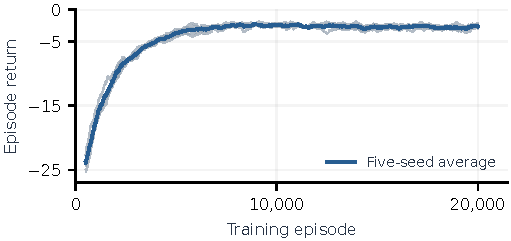
\includegraphics[width=\linewidth]{assets/training_measured.pdf}
\captext{\textbf{Fig. 1.} Actual exploration-policy training returns: 500-episode moving means for five independent runs (gray), with their average (blue). These are descriptive traces, not confidence intervals or final ensemble performance.}

Final testing uses 10,000 fresh scenarios $ 900000000+103i $, $ i=0,\ldots,9999 $, disjoint from known training/development/history. Configuration, checkpoints, comparison family and sample size froze before access. Shared exogenous noise pairs all policies by scenario. \InferenceMethod

\sect{6. Primary return and trade-offs}
\PrimaryResults

\SecondaryResults

Raw episodes, all family/fixed-checkpoint contrasts, per-seed metrics, source hashes and frozen manifests accompany the code. No legacy score from a different reward is used as a numerical benchmark.
\end{minipage}\hfill
\begin{minipage}[t]{.482\textwidth}\vspace{0pt}\small
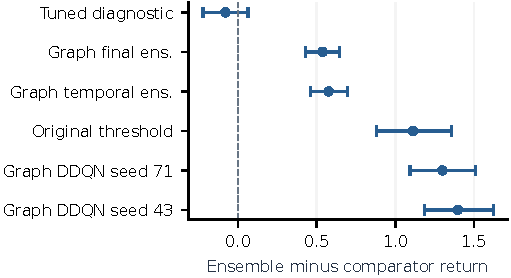
\includegraphics[width=\linewidth]{assets/comparison_measured.pdf}
\captext{\textbf{Fig. 2.} The six most limiting simultaneous return-difference bounds in the prespecified family. Points are ensemble minus comparator mean return; bars are Bonferroni-adjusted bootstrap intervals over all 55 primary contrasts, using 50,000 resamples and 10,000 shared scenarios. The ensemble's trained members are fixed.}

\begin{center}\footnotesize\setlength{\tabcolsep}{3.5pt}
\begin{tabular}{lrrrr}
\toprule
\textbf{Policy} & \textbf{Return} & \textbf{Crit.} & \textbf{False iso.} & \textbf{Conf.\%}\\
\midrule
\MetricTable
\bottomrule
\end{tabular}
\end{center}
\captext{\textbf{Table 1.} Final means. Critical hosts ever compromised and clean-host isolations are counts/episode. Confirmation is the mean within-episode fraction of infected hosts explicitly diagnosed. Secondary intervals are exploratory; complete estimates accompany the raw results.}

\sect{7. Fair comparison and scope}
The 22 comparator methods include previous corrected RL agents, original rules and tabular encoding, matched 20k-episode graph-dueling retraining (learned-only and prior/shield hybrid), temporal/final ensembles and a diagnostic threshold rule tuned over 40 validation configurations. Original checkpoints are clearly marked domain transfers: their lawful 58D adapter uses causal posterior marginals and public inspection history, with the unavailable privileged new-infection-count channel fixed to 0. Transfer and retraining are distinct.

For infected host $ i $, censored confirmation delay is $\min(t_i^{\rm confirm},T)-t_i^{\rm infection}$, with $\infty $ for unconfirmed hosts. Isolated but unconfirmed infections remain censored, so containment need not imply diagnosis. Coverage accompanies this measure. Controls with zero false isolation preclude a strict win on every metric.

The known synthetic model and $2^N$-state filter limit scalability and external validity. The shared head has restricted cross-host deployment context; several training/representation changes occur together, so results do not isolate one component's causal effect. Only one temporal ensemble is deployed: uncertainty is conditional on its fixed members, not variability across independently trained ensembles. Results establish a bounded comparison, not universal dominance or real-network effectiveness.

\vspace{2pt}{\footnotesize
\begin{thebibliography}{3}
\setlength{\itemsep}{1pt}\setlength{\parskip}{0pt}
\bibitem{pomdp} L.~P.~Kaelbling, M.~L.~Littman and A.~R.~Cassandra. Planning and acting in partially observable stochastic domains. \emph{Artificial Intelligence} 101:99--134, 1998. \href{https://people.csail.mit.edu/lpk/papers/aij 98-pomdp.pdf}{Author full text}.
\bibitem{ddqn} H.~van Hasselt, A.~Guez and D.~Silver. Deep reinforcement learning with Double Q-learning. \emph{AAAI}, 2016. \href{https://arxiv.org/abs/1509.06461}{arXiv:1509.06461}.
\bibitem{dueling} Z.~Wang et al. Dueling network architectures for deep reinforcement learning. \emph{ICML}, PMLR 48:1995--2003, 2016. \href{https://proceedings.mlr.press/v 48/wangf 16.html}{Publisher}.
\end{thebibliography}}
\end{minipage}
\end{document}
